\documentclass{standalone} 
\usepackage{tikz} 
\usepackage{pgfplots} 
\usepackage{xcolor} 
\usetikzlibrary{shapes,arrows,shadows,snakes,calendar,matrix,spy,backgrounds,folding,calc,positioning,patterns,hobby} 
\begin{document} 

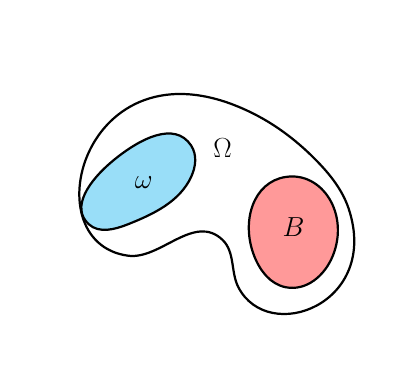
\begin{tikzpicture}[>=latex,scale=0.4,transform shape,label distance=-5,use Hobby shortcut ]

\path
  (0.5,-2.0) coordinate (z0)
  (4.0,0.5) coordinate (z1)
  (3.0,2.0) coordinate (z2)
  (1.0,3.5) coordinate (z3)
  (-3.0,-1.0) coordinate (z4)
  (0.0,-0.5) coordinate (z5); 
 \draw[black, thick,closed,thick,fill=white,fill opacity=1.0] (z0) .. (z1) .. (z2) .. (z3) .. (z4) ..(z5);
  

  \path
  (-3.0,0.0) coordinate (w0)
  (-1.0,1.5) coordinate (w1)
  (-1.0,2.5) coordinate (w2)
  (-3.5,2.0) coordinate (w3)
  (-4.25,-0.0) coordinate (w4);
  \draw[black, thick,closed,thick,fill=cyan ,fill opacity=0.4] (w0) .. (w1) .. (w2) .. (w3) .. (w4);

\path
  (2.0,-2.0) coordinate (v0)
  (3.5,-1.0) coordinate (v1)
  (2.0,1.5) coordinate (v2)
  (1.0,-1.0) coordinate (v3);
  \draw[black, thick,closed,thick,fill=red ,fill opacity=0.4] (v0) .. (v1) .. (v2) .. (v3);
  
  \draw[] ( 0 ,2.0 )  node[above]{ \Huge  \bf  $ \Omega$ };
  \draw[] ( -2.5 , 1.0 )  node[above]{ \Huge  \bf  $ \omega$ };
  \draw[] ( 2.25 , -0.5 )  node[above]{ \Huge  \bf  $ B$ };

\end{tikzpicture} 

\end{document} 
  \draw[line width=.2mm,draw=black,dotted] (3.0,2.0) circle [radius=4.5cm]; 
  \draw[line width=.2mm,draw=black,dashed] (3.0,2.0) circle [radius=6.5cm]; 
  
  %\draw[line width=1mm,draw=magenta] (3.0,2.0) circle [radius=5cm]; 
  %\draw[] ( 0.5 ,3.5 )  node[above]{ \Huge  $\Omega_{\mathrm{int}}$ };
 
  \draw [line width=.25mm,->] (3.0,5.5) --node[near start,right]{ \; \huge $ u_i$} (3.0,3.75); 
  \draw [line width=.25mm, decorate,decoration={expanding waves,angle=20},segment length=4.5pt ] (3.0,5.6) -- (3.0,4.2); 
  
  %\draw [decorate,decoration={expanding waves,angle=7},segment length=2pt]  (3.0,7.5) -- (3.0,4.0); 
    
   \draw [line width=.25mm,->] (2.5,0.0) --node[near start,left]{ \huge $ u_s$ \; \;} (1.5,-1.5); 
   \draw [line width=.25mm, decorate,decoration={expanding waves,angle=20},segment length=3.5pt] (2.5,0.0) -- (1.5,-1.5); 
   
   \draw [line width=.25mm,->] (3.5,0.0) --node[near start,right]{ \huge \; \; $ u_s$} (4.5,-1.5);  
   \draw [line width=.25mm, decorate,decoration={expanding waves,angle=20},segment length=3.5pt] (3.5,0.0) -- (4.5,-1.5);  


  \draw[] ( 2.75 ,1.5 )  node[above]{ \Huge  $K$ };
  
   \draw[] ( 0.0 ,2.75 )  node[above]{ \huge  $k(x)$ };
     
    %\draw[] (  3.0 ,7.0 )  node[above]{ \huge  $k = k( \vert x \vert)$ };
   %\draw[] ( -4.5 ,5.0 )  node[above]{ \huge  $k \equiv k_{\infty}$ };
  
  %\draw[] ( 0.5 ,3.5 )  node[above]{ \Huge  $\Omega_{\mathrm{ext}}$ };
   
 %\draw[decorate,decoration={expanding waves,angle=7}] (0,0)   -- (3,0);
